
\begin{minipage}{0.7\linewidth}
\section{Thyristoren}
Ein Thyristor besteh aus vier Halbleiterschichten d.h. aus drei pn-Übergängen\newline
Thyrisotren sind einschaltbare Bauelemente.\newline
Thyristoren sind  \" einschaltbare Dioden\". Thyristoren werden mit dem Zündimpuls der Zwischen Gate (G) und Kathode (K) kurzzeitig anliegt durchgeschalten.
\end{minipage}
\begin{minipage}{0.3\linewidth}
     \hspace{1cm}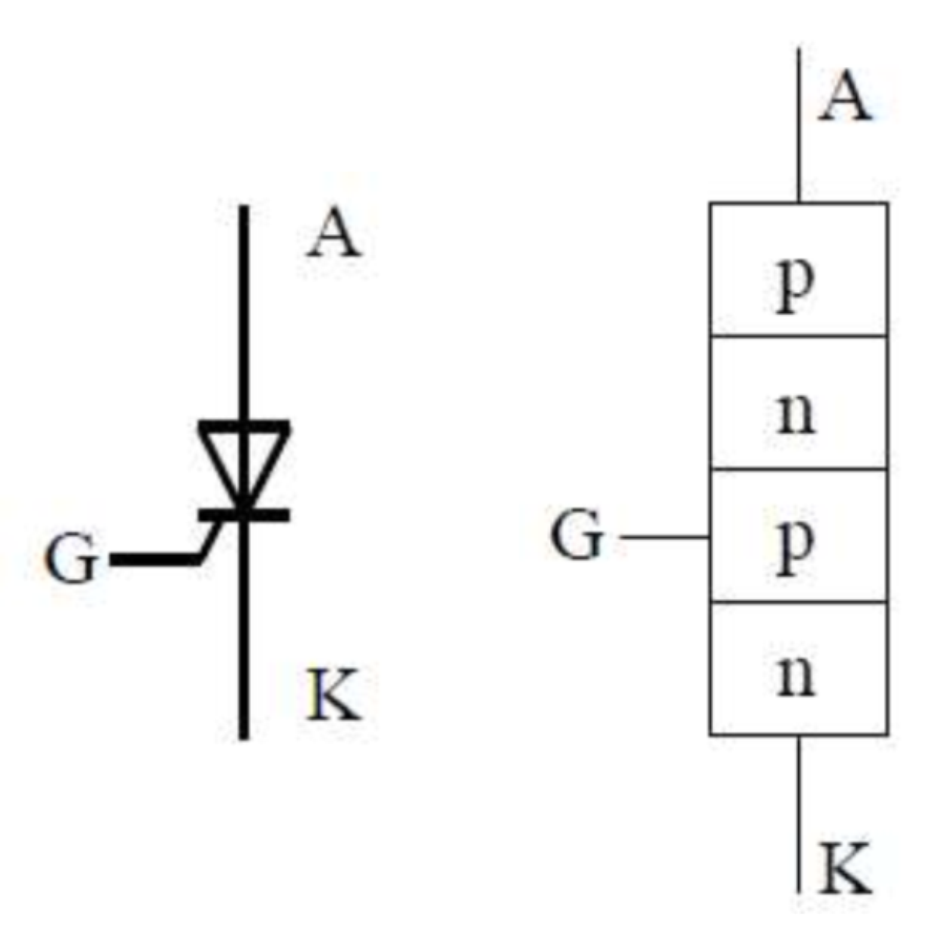
\includegraphics[width=0.5\linewidth]{images/thyraufbau}
\end{minipage}
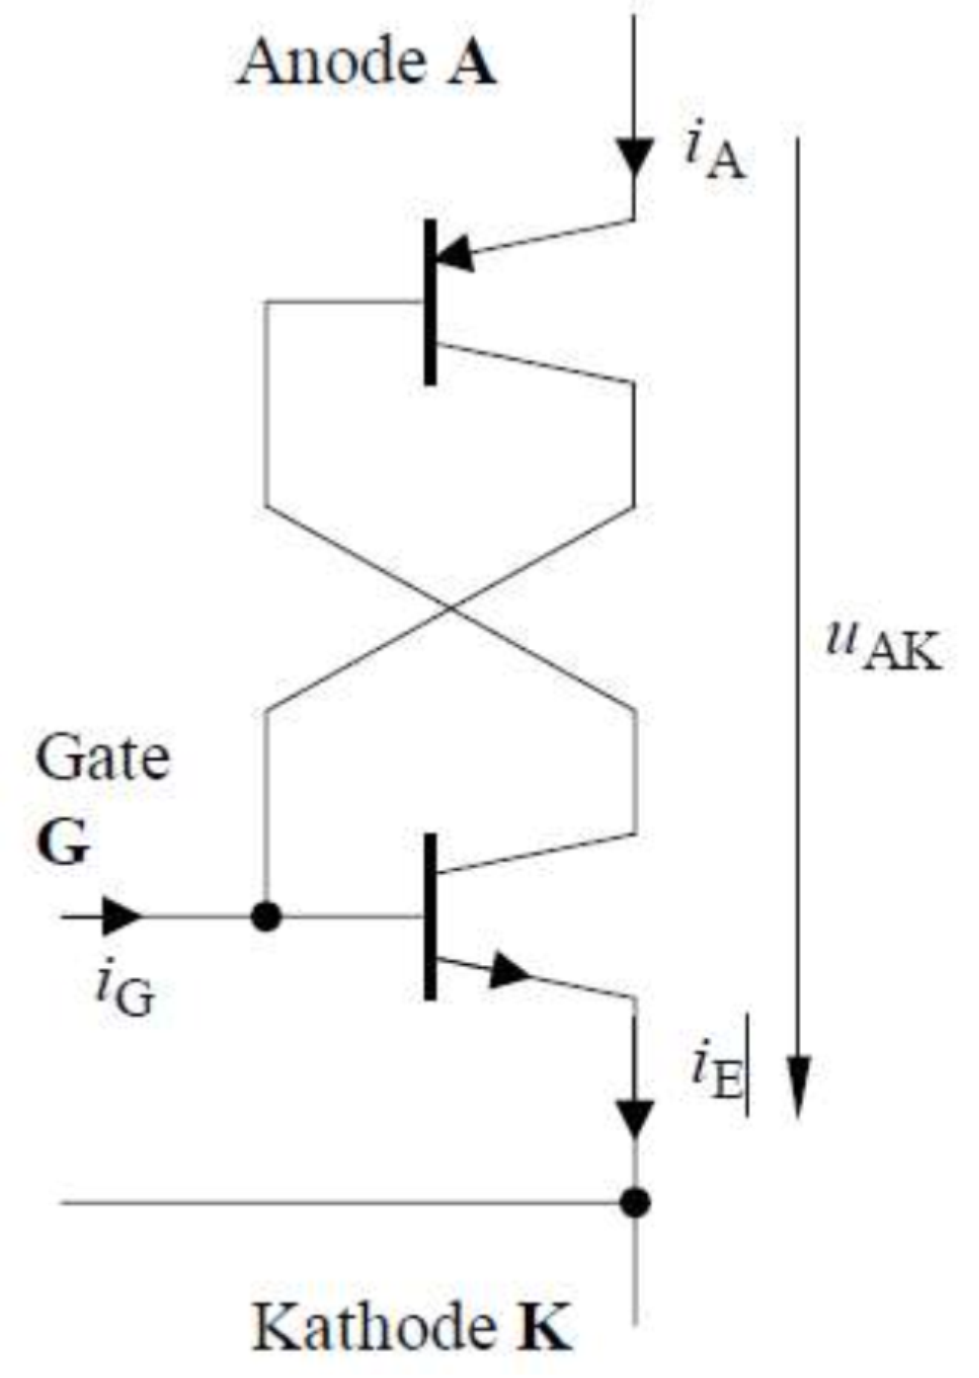
\includegraphics[width=0.15\linewidth]{images/thyrESB}
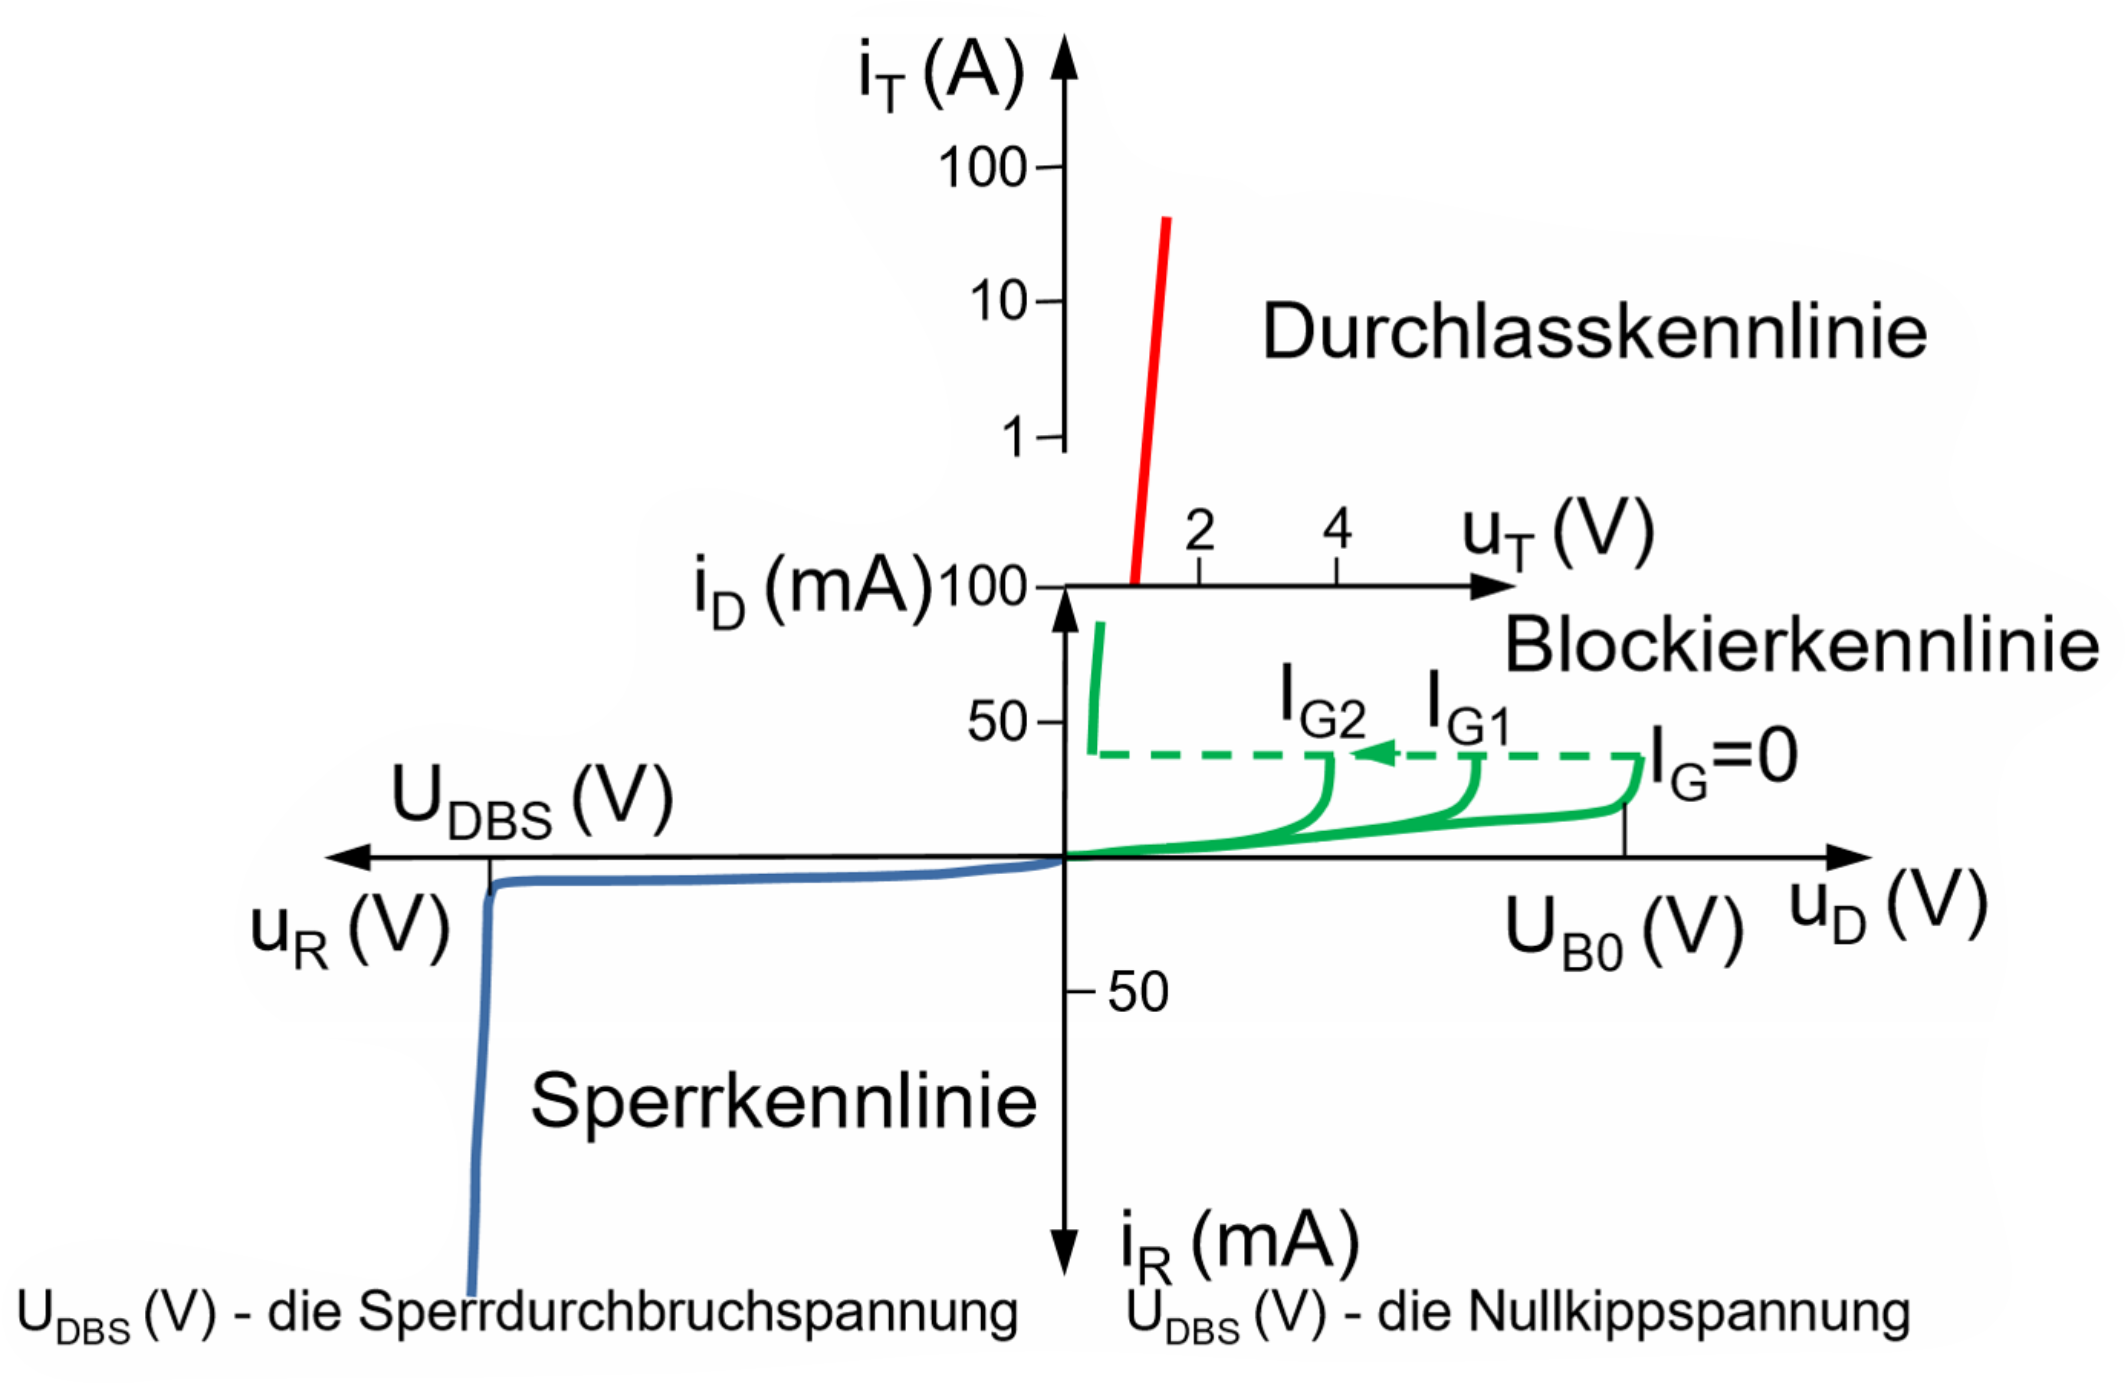
\includegraphics[width=0.4\linewidth]{images/thyrKennlinie}
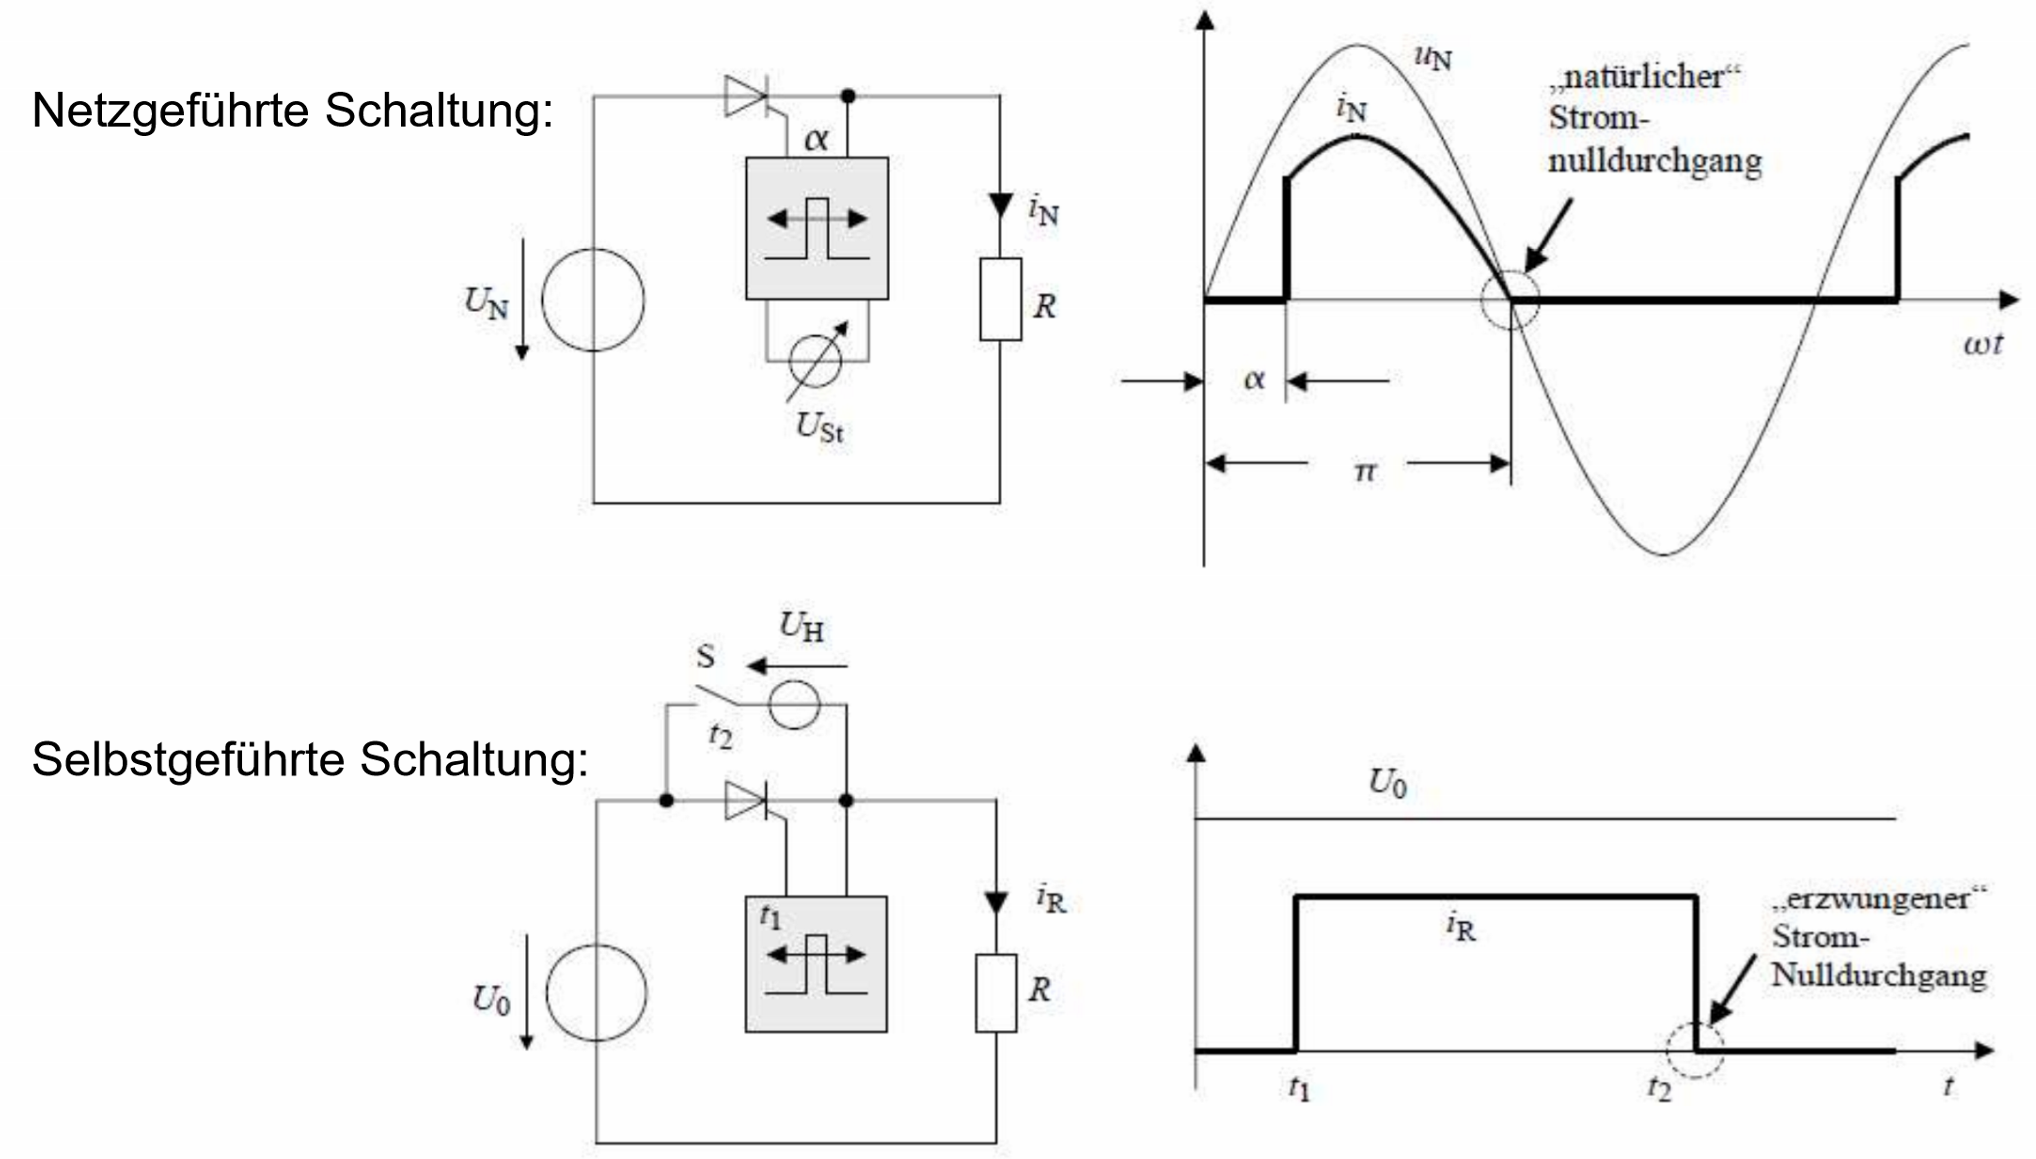
\includegraphics[width=0.45\linewidth]{images/thyrSchaltung}

\subsection{Thermische Eratzschaltung}
\begin{multicols}{3}
    \begin{minipage}{\linewidth}
        \textbf{Thermische Kenngrösse}\newline
        Wärmeleistung P [W]\newline
        Temperaturunterschied $ \vartheta $[K]\newline
        Wärmewiderstand $ R_{th} $ [${K}{W}$]\newline
        \textbf{Elektrische Kenngrösse}\newline
        Strom I  [A]\newline
        Spannung [V]\newline
        Widerstand [$\nicefrac{V}{A}$]\newline
    \end{minipage}

	\begin{minipage}{\linewidth}
		\subsubsection{Thyrisor ohne Kühlung}
		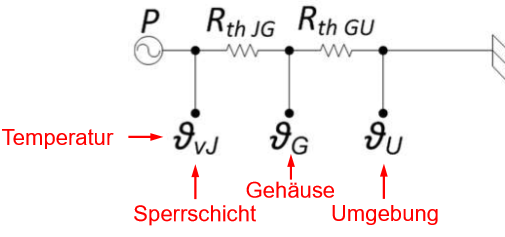
\includegraphics[width=\linewidth]{images/thyrOK}
		\[ \vartheta_{vJ}-\vartheta_U=P \cdot (R_{th\; JG}+R_{th\; GU}) \]		
	\end{minipage}

	\begin{minipage}{\linewidth}
		\subsubsection{Thyrisor mit Kühlung}
		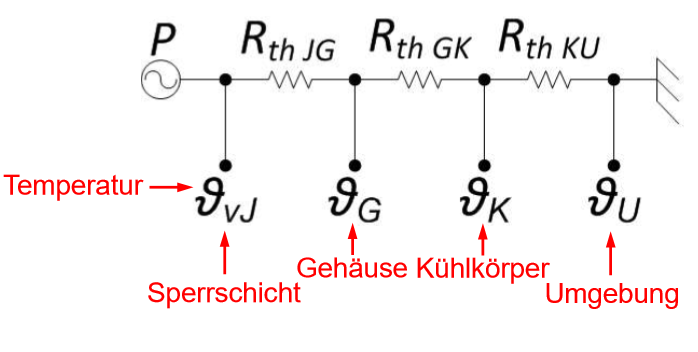
\includegraphics[width=\linewidth]{images/thyrMK}
		\[ \vartheta_{vJ}-\vartheta_U=P \cdot (R_{th\; JG}+R_{th\; GK}+R_{th\; KU}) \]	
        \[ R_{th \; KU}=\dfrac{\Delta \vartheta}{P} \]
	\end{minipage}
\end{multicols}

\vspace{-1.5cm}
\textbf{Beispiel Schaltverluste bei B2C}\newline
\begin{tabular}{ll}
    Spitzenwert des Thyristorstromes&
    $\hat{I}_{R} = \frac{\hat{U}_{2}}{R}$\\
    \\
    
    Mittelwert des Thyristorstromes &
    $I_{T AV} = \frac{1}{2\pi}\int\limits_{\alpha}^{\pi}I_{Rm} \cdot sin(\beta) \cdot \diff\beta= \frac{\hat{I}_{R}}{2\pi} \cdot (1+cos\alpha)$\\
    \\

    Effektivwert des Thyristorstromes &
    $I_{T RMS} = \sqrt{\frac{I_{RM}^2}{2\pi}\int\limits_{\alpha}^{\pi}sin^2(\beta)\diff\beta}= \frac{\hat{I}_{R}}{2}\sqrt{\frac{\pi - \alpha}{\pi}+\frac{sin2\alpha}{2\pi}}$\\

    momentane Verlustleistung:&
    $p(t) = u_{T}(t) \cdot i_{T}(t)$\\
    Mittelwert der Verlustleistung: &
    $P_{T} = \frac{1}{T}\int\limits_{0}^{T}u_{T}(t) \cdot i_{T}(t) \cdot \diff t = U_{T0} \cdot \frac{1}{T}\int\limits_{0}^{T}i_{T}(t)\diff t+r_{T} \cdot \frac{1}{T}\int\limits_{0}^{T}i_{T}^2(t)\diff t$\\
    \\
    & $P_{T} = U_{T0} \cdot I_{T AV} + r_{T} \cdot I_{T RMS}^2$\\
\end{tabular}

 $I_{T AV}$ ist der Mittelwert und $I_{T RMS}$ der Effektivwert des Thyristorstroms\newline
\textbf{Der Wert für $U_{T0}$ kann aus dem Datenblatt des Thyristors herausgelesen werden.}

\begin{minipage}{0.5\linewidth}
    \subsection{Abschaltbarer Thyristor}
    \begin{minipage}{0.7\linewidth}        
        \textbf{(GTO = Gate-Turn-Off)}\newline
        Der GTO Schaltet aus, wenn ein ausreichend hoher nagativer Gate-Strom auftritt.\newline
        Amplitude des Gate-Stromes muss 20\% bis 30\% des abzuschaltenden GTO-Stromes betragen.
    \end{minipage}
    \begin{minipage}{0.2\linewidth}
        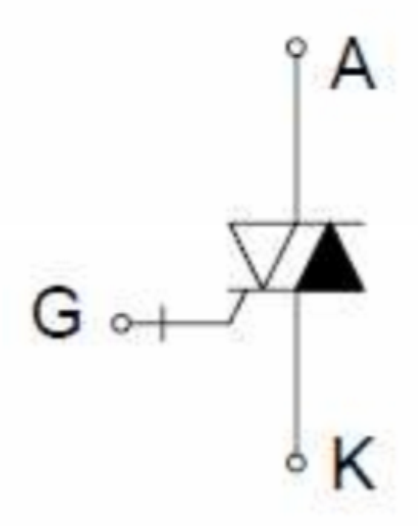
\includegraphics[width=\linewidth]{images/GTOSymbol}
    \end{minipage}    
\end{minipage}
\begin{minipage}{0.5\linewidth}
    \subsection{IGCT}
    \begin{minipage}{0.7\linewidth}
        \textbf{Integrated Gate-Commutated Thyristor}
        IGCT sind die Weiterentwicklung der GTO.\newline
        Sie werden hauptsächlich für Mittelspannungsumrichter iengesetzt.
    \end{minipage}
    \begin{minipage}{0.2\linewidth}
        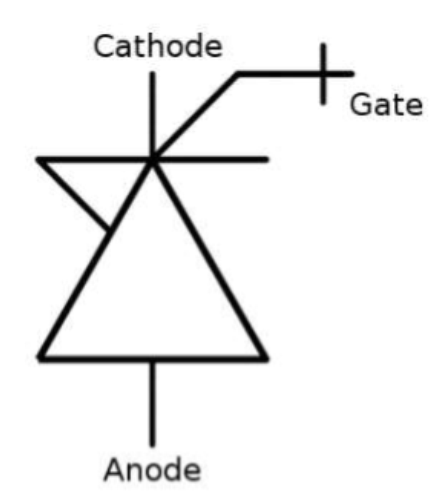
\includegraphics[width=\linewidth]{images/IGCTSymbol}
    \end{minipage} 
\end{minipage}
\clearpage
